\newcommand{\ClassPath}{../../yukibook.cls}
\documentclass{\ClassPath/yukibook}


\begin{document}

    \yukibook{Cómo hacer una buena documentación} % Title
    {Rubén Gómez Olivencia}  % Author
    {2023-09-02}    % Year
    {Formación Profesional: \linebreak Informática y Comunicaciones} % Name of degree
    {O al menos intentarlo} % catch phrase
    {} % the phrase's author
    {img/portada.png} %cover
    {006c8c}
    {pfsense} %mini-title

    \coverpage
    \graphicspath{{../../yukibook.cls/}}
    \licensepage

    \tableofcontents

    %--------------------------------------------------------------------------
    % Start your parts, chapters and sections here
    %--------------------------------------------------------------------------
    \graphicspath{{img/documentacion/}}
    \chapter{Introducción}

En nuestra vida laboral nos va a tocar realizar proyectos que consistirán en buscar soluciones a problemas y que conllevará una serie de tareas técnicas que tendremos que realizar: configurar una red de ordenadores, modificar una aplicación web, crear una aplicación móvil, ...

Junto a ese proyecto lo más habitual es que se acompañe de una documentación del proyecto realizado, en el que se deberá explicar cuáles han sido las decisiones tomadas y cómo se ha realizado el proyecto.

Aunque hayamos leído cierta documentación en internet, como no estamos acostumbrados a realizar nuestra propia documentación, cuando comenzamos a crear documentación propia el resultado final que obtenemos no suele ser el adecuado.

Es por eso que en este documento se van a dar una serie de consejos y pautas para realizar una buena documentación.


\chapter{Lenguaje formal/técnico}

\begin{minipage}{0.7\linewidth}
%    TODO: crear environment para minipage
    \setlength{\parskip}{1.2em}
    \renewcommand{\baselinestretch}{1.4}
    Aunque pueda parecer obvio, en las documentaciones no se puede utilizar un lenguaje coloquial, por lo que debemos escribir siempre desde un punto de vista técnico.

    Se debe utilizar lenguaje formal y cuando hagamos referencia a opiniones, pensamientos o decisiones \textbf{se hará uso del plural mayestático}:
\end{minipage}
\hfill
\begin{minipage}{0.2\linewidth}
    
\includegraphics[width=0.7\linewidth]{debian.png}
\end{minipage}



\infobox{\textbf{Creemos que la solución realizada en este proyeto es la adecuada porque ...}}


De esta manera se evita que la persona que escribe sea la que dé su opinión, y de esta manera el documento da la sensación que se ha realizado por un grupo de personas, que se ha tenido en cuenta la opinión de otros, o que ha sido supervisado.

Cuando se haga uso de opiniones o se indique unos ajustes “\textbf{mejores que otros}” siempre deben llevar su justificación asociada para que se entienda el por qué de la elección realizada.

\errorbox{\textbf{Por supuesto, es muy importante que el documento no cuente con faltas de ortografía, frases inacabadas, inconexas, ...}}


\chapter{Formato del documento}
Aunque parece sencillo, el estilo puede resultar lo más difícil de realizar, por lo que tenemos que seguir una serie de consejos, que se expondrán a continuación, pero que no tienen por qué ser los únicos.


\section{Letra, sangrías y ajustes del documento}
Hoy en día, la mayoría de editores de texto \textbf{WYSIWYG} (del inglés “\textit{What You See Is What You Get}”, lo que ves es lo que obtienes), como pueden ser Microsoft Word, LibreOffice o Google Docs, tienen unas opciones por defecto que hace que los documentos queden visualmente atractivos y que en principio no tengamos que modificar muchas cosas.

Aún así, modificar estas preferencias es sencillo y puede hacer que el documento quede mejor, personalizado a nuestro gusto y se diferencie de los demás.

\infobox{\textbf{En las empresas se suelen crear plantillas personalizadas, con el logotipo de la empresa, colores corporativos, tipos de letra utilizados en el logo, ...}}


Tal como se puede ver en este documento, el interlineado y la separación entre párrafos facilita la lectura del mismo, por lo que debería ser una configuración a ajustar.

\begin{center}
    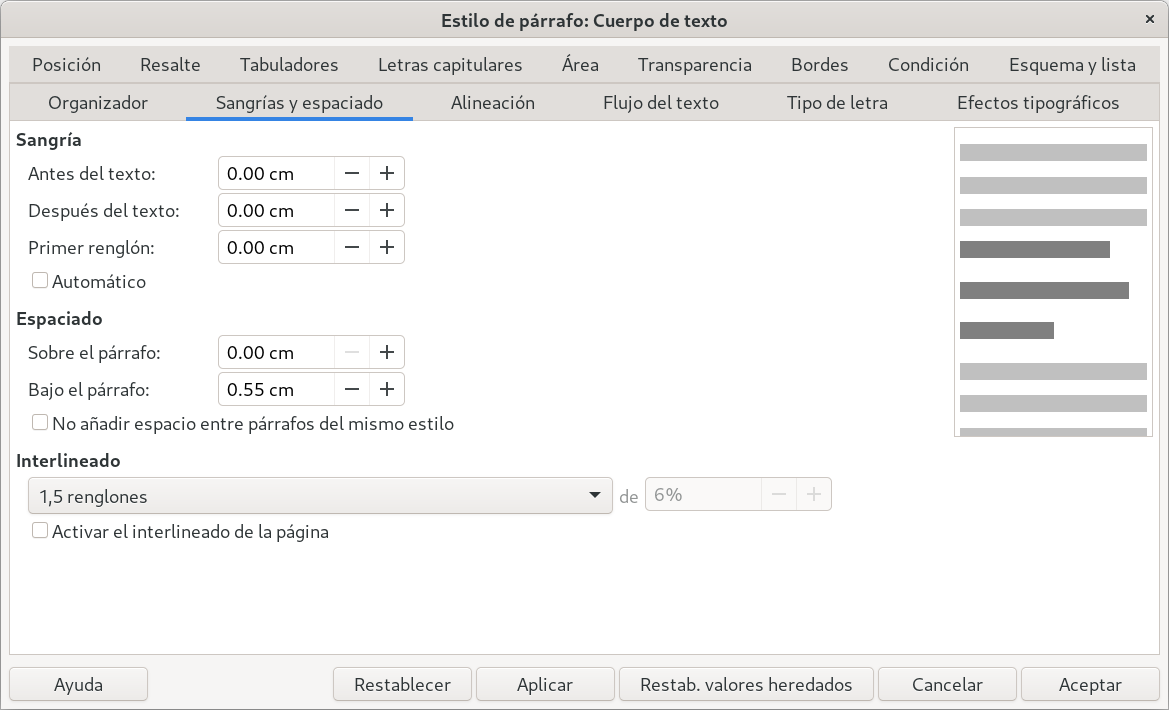
\includegraphics[width=0.7\linewidth]{libreoffice.png}
\end{center}

Cada editor de texto tiene unos ajustes que se pueden modificar, por lo que es recomendable dedicar un tiempo para entender las distintas configuraciones que ofrece. En la imagen superior se puede ver la configuración que ofrece \href{https://es.libreoffice.org/}{Libreoffice}


Es importante modificar los ajustes de cada estilo y no ir título a título o párrafo a párrafo. Si queremos que todos los “Título 1” sean de color verde y tamaño 15 debemos editar ese estilo. Si luego decidimos que pasen a ser de color azul, con cambiar el estilo nos modificará todos los títulos y así no tendremos que ir uno a uno.

\infobox{\textbf{Si modificamos las configuraciones de un estilo, se aplicará a todo texto que sea de ese estilo en el documento.}}
\vspace{10pt}

\subsection{Aspecto visual general}
Tal como se puede apreciar en este documento, no hacen falta grandes florituras para que un documento quede atractivo a la vista y sea sencillo de leer.


\begin{minipage}{0.19\linewidth}
    
\includegraphics[width=0.65\linewidth]{debian.png}
\end{minipage}
\hfill
\begin{minipage}{0.8\linewidth}
    \setlength{\parskip}{1.2em}
    \renewcommand{\baselinestretch}{1.4}
\textbf{Hay que tener ojo crítico con nuestros propios documentos} y realizar una comparación con el trabajo realizado y con otros documentos que hayamos visto.


Si nuestro documento no tiene las características exigidas, o a nosotros mismos nos parece que no resulta atractivo, no es raro pensar que al profesor que lea el documento tampoco le guste.
\end{minipage}

El aspecto visual puede cambiar la predisposición del lector, ayudando a que la lectura sea más agradable y sencilla. Y al contrario, puede predisponer a no querer seguir leyendo y terminar cuanto antes el documento.

\section{Cabecera, pie de página y números de página}
Es recomendable añadir el número de página en el documento, ya que facilita saber en qué parte del documento nos encontramos y para de esta manera poder hacer referencia a una página concreta.

Normalmente el número de página suele aparecer en el pie de página, como se ha hecho en este documento.

Aparte, se puede añadir el título del documento, el nombre de la empresa o algún tipo general en el pie de página o en la cabecera. Lo que es importante es que en estos apartados el tamaño de letra utilizado sea menor al del texto general y que haya la suficiente separación como para que no se mezcle con el texto.

Una vez más, se recomienda ser crítico con lo realizado, comprobar que el aspecto visual general de lo realizado es acorde y facilita la lectura.


\section{Imágenes y su composición}

En los documentos en los que hay que añadir imágenes hay que tener en cuenta cómo se va a realizar la composición, el tamaño de las imágenes y dónde situarlas.

\subsection{Tamaño y posicionamiento}
Dependiendo de la imagen que queramos utilizar, podríamos ajustarla al centro, ocupando gran parte de la zona central del documento, como ya hemos visto más arriba, o como es el ejemplo que se muestra a continuación.

\begin{center}
    \includesvg[width=0.7\linewidth]{debian.svg}
\end{center}

En este caso es el nombre de la distribución \href{https://www.debian.org/}{Debian}, pero anteriormente hemos visto una captura de pantalla de un programa.

\subsection{Explicación sobre las imágenes}
A lo largo de este documento se han añadido ciertas imágenes que se han puesto de distintos tamaños tanto a la izquierda como a la derecha de párrafos.

Estas imágenes han sido un mero ejemplo de cómo se pueden poner imágenes que acompañan al párrafo, siempre dentro de los márgenes del documento y dejando espacio al texto.

Toda imagen que sea añadida al documento debe llevar consigo una explicación de a qué se refiere con ella. En el caso de las imágenes al lado de los párrafos, los párrafos harán referencia a las imágenes. En el caso de imágenes centradas, antes o después de la misma se deberá explicar a qué hace referencia


Por ejemplo:

\begin{quote}
“Una vez realizado el paso anterior llegaremos a la siguiente ventana que nos indicará los parámetros que una vez rellenados podremos hacer click en el botón \textbf{siguiente}.”
\end{quote}

\subsection{Recorte de imágenes}
Cuando en una imagen queremos hacer referencia a algo en concreto, lo ideal es no poner la captura de pantalla del escritorio completo, sino sólo hacer referencia a la ventana de la que estamos hablando.

Con esto conseguimos hacer que la atención se centre sobre lo que es realmente importante, y que no aparezca información visual que no es necesaria. Si queremos concretar algo dentro de una imagen, es recomendable bordear esa sección de un color (rojo, por ejemplo) para que sea más apreciable.

También es conveniente añadir un pequeño borde a ciertas imágenes, ya que en los escritorios actuales las ventanas hacen uso de fondo blanco y no se vería de manera correcta con el fondo blanco del documento.

A continuación se visualiza la misma imagen con y sin borde:

\begin{center}
    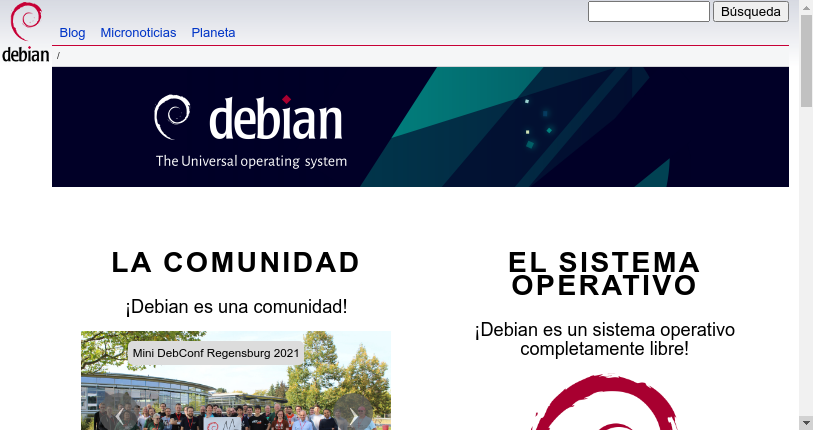
\includegraphics[width=0.45\linewidth]{captura.png}
    \hfill
    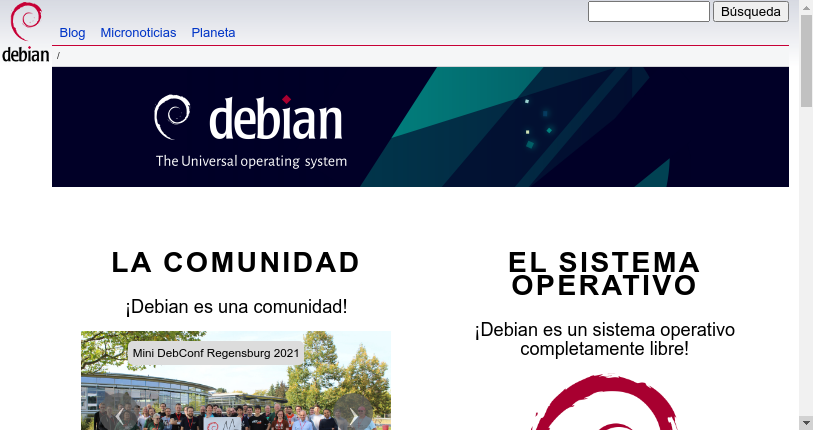
\includegraphics[frame,width=0.45\linewidth]{captura.png}
\end{center}

Como se puede apreciar, la imagen que no tiene borde hace un efecto de “continuidad” que puede dar a equivocación de cuándo empieza la imágen y cuándo termina.

\infobox{\textbf{Es recomendable poner un borde a las imágenes (como capturas de pantalla con fondo blanco).}}


\chapter{Referencias}
En todo documento puede existir referencias a otro texto, o texto copiado y/o adquirido de varias fuentes, y en caso de ser así debe de ser referenciado.

\vspace{-10pt}
\begin{quote}
    “Las referencias a otras obras son una parte muy importante en la literatura de muchas profesiones; cada una de ellas ha diseñado su propia manera de incluir esta información en el texto, y estas han dado lugar a formatos estandarizados de cita.” (Fuente: \href{https://es.wikipedia.org/wiki/Wikipedia:Referencias}{Wikipedia})
\end{quote}


Tal como se puede ver en el párrafo anterior, el texto está entrecomillado, con una sangría superior y al final del mismo aparece la fuente donde se ha cogido la información y un enlace a la web de referencia. Existen distintas maneras de referenciar textos o citas de otros documentos, pero no entraremos en detalle sobre ello.


Por tanto, si a la hora de crear un documento hacemos referencia a otros textos, deberíamos indicarlo, y más cuando hacemos corta-pega del mismo. Hay que ser objetivos y dar a conocer al lector que lo que acaba de leer no es de elaboración propia y que por tanto se ha utilizado el texto de otro autor. De ahí que haya que referenciar al autor original o la página web de donde se ha sacado la información.

Otro ejemplo podría ser: tal como escribió \href{https://es.wikipedia.org/wiki/Isaac_Newton}{Isaac Newton} a Hooke: “\textit{Si he visto más lejos es porque estoy sentado sobre los hombros de gigantes.}”, lo que viene a decir que hasta él mismo había basado sus estudios y había conseguido sus logros haciendo uso de las aportaciones de otros grandes científicos anteriores. Como se puede ver, la referencia está entre comillas también y en tipo de letra itálica.


\chapter{Elementos de un documento}

Un documento técnico debe contar con los siguientes elementos.

\section{Portada}
Un documento técnico debe contar con una portada en la que se puede añadir una imagen sobre lo realizado, el nombre/logo de la empresa junto con el nombre/logo del cliente... Aquí dependerá de la plantilla corporativa.

En la portada también se deben añadir los nombres de las personas que han realizado el documento y la fecha de realización.


\section{Índice}

Se ha añadido un índice al inicio del documento en el que aparecen reflejados los títulos y las páginas en las que aparece.

\textbf{Este índice se realiza de manera automática por el editor de texto}, por lo que mostrará las páginas donde aparece cada título. En caso de haber cambios en el documento, el índice se debe de actualizar para que refleje los nuevos capítulos, páginas, ...


\section{Introducción}
Al igual que se ha realizado en este documento, debe haber una introducción que indique lo que se va a explicar a lo largo de todo el documento.

En un documento técnico también se suele añadir cuáles han sido las funciones de los componentes del grupo que ha llevado a cabo el proyecto.

\section{Parte central}
Es la parte del documento donde se detalla lo realizado en el proyecto. Se debe separar en capítulos, secciones, subsecciones... es decir, crear una jerarquía en el documento.

Esta jerarquía de secciones se realiza a través de los distintos tipos de “títulos” que nos proveen los editores de texto, y que se ve muy bien reflejado en el índice.


\section{Resumen/Conclusiones}
En las documentaciones se añade un resumen final en donde se reflejan los aspectos más importantes que se han detallado en ella.

Este apartado suele estar al final, en una hoja separada, y como su propio nombre indica, trata de resumir los aspectos más importantes del mismo.

También es una oportunidad de \textbf{dar valor a lo realizado, mostrando al clientes los puntos fuertes}, para dejar una imagen positiva de lo realizado. \textbf{Esto puede ayudar a futuras contrataciones}.

\end{document}
